\chapter{Implémentation - Etude de l'art}

  \section{Choisir ses outils}
  Une Plate-forme d'Intégration Continue (PIC) peut être mise en place avec un nombre incalculable d'outils différents. Il est important de comprendre la finalité et les caractéristiques de l'Intégration Continue que l'on souhaite mettre en place afin de choisir au mieux ses outils. L'Intégration Continue de base, peut être mise en oeuvre avec un ensemble très simple d'outils maisons mais généralement dans un environnement d'entreprise il est préférable d'utiliser les outils adoptés et soutenus par la communauté.

    \subsection{Scaling}
    Comme nous l'avons vu dans la section~\ref{Features of Continuous Integration}, l'Intégration Continue peut être mise en oeuvre en utilisant uniquement le contrôle de version, les scripts de build, un appel périodique à ces derniers et les emails. Cela peut s'avérer suffisant pour un projet simple, composé de quelques éléments, mais lorsque la quantité des composants buildables augmente cela peut dévenir un veritble cauchemar du côté de la maintenance. Pour résoudre ce problème de mise à l'échelle, un bon serveur d'Intégration Continue est indispensable. L'utilisation et la configuration d'un serveur d'Intégration Continue fourni par une société tierce est une tâche relativement triviale grâce à l'interface utilisateur graphique (GUI) mise à la disposition des développeurs.\\

    Lorsque le nombre de builds, la quantité de code à compiler et le nombre de tests à exécuter augmentent, la puissance de calcul nécessaire augmente parallèlement. Afin d'accroitre la puissance de traitement de notre serveur d'Intégration Continue, on peut étendre, dans certaines limites, la quantité de coeurs de son processeur (CPU) - scalabilité verticale - ou augmenter le nombre de serveurs physiques dédiés à la PIC - scalabilité horizontale. Cette scalabilité horizontale est aussi nécessaire lorsque que la build à besoin de s'exécuter sur différents environnements ou plates-formes.

    \subsection{Le choix du serveur d’Intégration Continue}

      \subsubsection{Support du langage de programmation}
      Il existe divers serveur d'Intégration Continue, chacun porté par une entreprise informatique différente. Certains d'entre eux sont conçus pour ne fonctionner qu'avec des langages de programmation spécifiques tandis que d'autres sont génériques et fonctionnent avec tous. Si l'entreprise dispose d'un parc informatique uniforme dans le langage et ne compte en déroger la première option peut être viable dans le cas contraire l'entreprise devra se tourner vers un serveur d'Intégration Continue générique.

      \subsubsection{Support du référentiel de code source}
      De même que pour le langage de programmation, le support du référentiel de code source doit être pris en compte lors du choix du serveur d'Intégration Continue. Nous distinguons deux mécanismes de communication entre le référentiel et le serveur; les Agents et les Webhooks.\\

      Les agents sont des modules, intégrés (dans le cadre d'un serveur propriétaire) ou non (dans le cadre de l'open source), qui effectuent, en toute transparence pour l'utilisateur, le lien entre le référentiel et le serveur. Leur utilisation est extrèmement simple et ne nécessite que très peu de configuration. L'inconvénient des agents est que si votre gestionnaire de code source n'est pas pris en compte, il est dès lors impossible d'utiliser ce serveur avec votre référentiel dans le cas d'un logiciel propriétaire ou très coûteux de développer votre propre agent dans le cas d'un serveur d'Intégration Continue open source.\\

      La majorité des serveurs d'Intégration Continue proposent un second mécanisme de communication avec le référentiel de code source via les Webhooks. Les webhooks servent à notifier des éléments externes à une application web qu'un événement a eu lieu sur celle-ci. Les serveurs d'Intégration Continue s'assurent ainsi d'être agnostiques du référentiel. Cependant votre gestionnaire de code source doit lui aussi implémenter les Webhooks pour pouvoir notifier le serveur.

      \subsubsection{La gestion des builds}
      Un des points importants à prendre en compte lors du choix de son serveur d'Intégration Continue est sa gestion des builds. Le déclenchement des builds, la possibilité d'exécutions parallèles, la gestion des dépendances interprojets, etc, sont propres à chaque serveur. Il est intéressant d'étudier chacune de ces spécificités afin de choisir l'outil le plus adéquat à vos besoins.

      \subsubsection{Extensibilité}
      Dans le cas ou aucun serveur d'Intégration Continue ne répond par défaut à l'intégralité de vos besoins, un serveur qui peut être étendu avec des plugins ce révèle être un bon choix. Avec ce mécanisme de plugin, pratiquement tout outil peut être intégré. Vous trouverez sur internet une quantité de plugin en fonction de votre serveur d'Intégration Continue. Vous êtes aussi libre de créer le votre et de le proposer à la communauté.

      \subsubsection{Autres caractéristiques}
      Les serveurs d'Intégration Continue ont un large éventail de caractéristiques que nous n'avons pas encore abordé mais qui doivent être pris en considération lors de votre choix.
      \paragraph{La publication} La publication regroupe la création des rapports et des artefacts ainsi que leur gestion. La méthode de base pour publier est l'email. Certains serveurs supportent également le Secure Copy (SCP), le protocole de transfert de fichier (FTP), les flux RSS...
      \paragraph{L'interface utilisateur} La caractéristique la plus visible des serveurs d'Intégration Continue est son interface utilisateur. La tendance est d'avoir une interface web. Rassurer-vous tous les serveurs en proposent une, ce qui fait la différence est, ce qui peut être fait à travers elle.
      \paragraph{Le suivi de problèmes} Si vous utilisez un outil de suivi de problèmes tel que Jira ou Bugzilla vous pouvez l'intégrer directement dans votre serveur d'Intégration Continue, dans la mesure ou votre serveur dispose d'un agent ou d'un plugin pour.
      \paragraph{L'environnement de développement} Certains serveurs d'Intégration Continue peuvent être intégrés aux environnements de développement (IDE). Pour cela votre IDE doit disposer d'un plugin pour votre serveur. Avec de tels plugins les status de vos builds peuvent être vus directement à partir de l'IDE sans avoir accès à l'interface graphique de votre serveur.

      \subsubsection{Installation et configuration}
      Un serveur d'Intégration Continue peut être installé de multiple façons. Pour les environnements Windows, presque tous les serveurs fournissent un installateur qui exécutera toutes les mesures nécessaires afin que vous disposiez d'une installation fonctionnelle. Pour les autres environnements les serveurs d'Intégration Continue soumettent des distributions autonomes tel que les paquets Debian ou les Web Archive (WAR). De ce cas, avant toute installation, vous devez vérifier les dépendances additionnelles (sdk, framework, ...) mentionnées dans le guide d'installation.\\

      Une fois l'installation effectuée le serveur d'Intégration Continue doit être configuré. La plupart des serveurs fournissent une interface graphique pour cela. Vous devrez en autre définir l'emplacement et le type de votre référentiel de code source, les outils de build, les contrôles d'accès... L'intégralité des serveur, même ceux possédant une interface graphique, sauvegarde vos configurations dans des fichiers ou dans des bases de données. Votre configuration peut ainsi être archivée, partagée et réutilisée.

      \subsubsection{Autres questions à considérer}
      \paragraph{Les coûts} Les coûts de mise en place et de maintenance du serveur d'Intégration Continue est un point à prendre en compte lors de votre choix. Il existe des serveurs gratuits - open source - (Jenkins) et des serveurs payants - propriétaire - (Visual Studio Team Services). Les serveurs open source sont libres d'utilisation mais ne proposent bien souvent pas de support technique. A l'inverse les serveurs payants nécessitent une licence d'utilisation mais fournissent un support technique, une expertise ainsi qu'un accompagnement.

      \paragraph{La communauté} Les serveurs d'Intégration Continue largement diffusés disposent d'une forte communauté active. Les solutions aux problèmes d'installation et de configuration courants sont généralement disponibles sur internet. De plus une communauté active pourra répondre à vos questions spécifiques. Une bonne communauté en ligne peut être une substitution aux supports techniques.

  \section{Logiciels et outils utilisés au sein de la DSI d'AXA France}
  Depuis maintenant 3-4 ans la DSI d'AXA France dispose d'une équipe dédiée à la mise en place, la maintenance et l'accompagnement des équipes dans l'Intégration Continue. Encore en phase de développement seuls quelques projets bénéficient de cette évolution. Dans la suite de ce mémoire nous prendrons en compte que les langages prédominants dans le parc applicatif d'AXA qui sont le Java, le C\# et le Javascript.

    \subsection{Serveur d’Intégration Continue}
    Historiquement, au sein d'AXA, deux grands langages composent essentiellement l'ensemble du socle applicatif web de l'entreprise; le Java (J2EE) et le C\# (.NET). Le choix du groupe c'est tourné vers l'utilisation de deux serveurs d'Intégration Continue distincts. Un serveur basé sur la suite Microsoft Visual Studio Team Services (VSTS) pour les applications .NET et un serveur basé sur le produit open source Jenkins pour les applications J2EE, Javascript ...\\

    De part son background informatique, AXA est attaché aux solutions proposées par Microsoft. La synergie des technologies Microsoft et son support technique offrent aux entreprises une garantie non négligeable quant à la qualité de ses services. C'est tout naturellement qu'AXA c'est dirigé vers leur serveur d'Intégration Continue Visual Studio Team Services 2010 pour les applications liées à l'environnement Microsoft - applications développées en .NET et déployées sur des serveurs Windows. Cependant, la version de VSTS 2010 ne supportait pas l'intégration et le déploiement de langages autres que ceux portés par Microsoft (depuis la version 2015 si). AXA a donc dû se tourner sur une autre solution pour le reste de ses applications.\\

    Jenkins est le leader des serveurs d'Intégration Continue open source. Développé en Java, il peut aussi bien être déployé dans un environnement Windows que Linux. De plus Jenkins et sa communauté proposent une pléthore de plugin afin d'intégrer facilement Jenkins dans votre environnement de travail. AXA c'est donc orienté vers cette solution pour ces applications Java et Javascript. Mais si Jenkins fournit les plugins nécessaires à l'intégration et au déploiement des applications .NET, pourquoi AXA propose la solution VSTS à ses équipes C\#?\\

    Jenkins est un produit développé en Java et open source, dans la plupart des cas il est installé sur un serveur Linux et configuré via son interface web administrative. Si vous déployez vos applications sur des serveurs Linux pas de problème. Toutefois, si votre application requiert une compilation .NET le problème se corse. La communauté met à disposition le plugin MSBuild pour palier à cela. Cependant celui-ci requiert une dll (de même nom) et étonnamment Microsoft ne propose pas de distribution Linux pour cette dernière. Il est toujours possible d'exécuter la dll MSBuild avec une surcouche WINE ou Mono mais le défis technique se révèle être une perte de temps dans la plupart des cas.
    Une alternative serait d'installer Jenkins sur un serveur Windows, et dans ce cas aucun problème d'intégration et de déploiement du côté des applications .NET. Nous aurions ainsi une PIC unique pour toutes nos applications. Néanmoins AXA à pour volonté de rester dans un écosystème Microsoft pour les applications .NET. Nous nous retrouvons ainsi avec 2 plate-formes d'Intégration Continue, une tournant sur Visual Studio Team Services 2013 et une sur Jenkins 1.2.\\

    \begin {boxedminipage} {11cm}
      Dans la suite de ce mémoire nous étudierons exclusivement la plate-forme d'Intégration Continue basée sur Jenkins.
    \end {boxedminipage}\\

    \subsection{Logiciel de gestion de version}
    Au moment ou j'écris ce mémoire, une grande migration du référentiel de code source à lieu à AXA. L'ancien outil, ClearCase - propriété d'IBM - est abandonné au profit de Team Foundation Server (TFS) - propriété Microsoft. Toutes les nouvelles applications, et donc celles impactées par l'Intégration Continue, ont officiellement pour gestionnaire de version cible TFS. Cependant quelques projets sont hébergés sur d'autres référentiels de code source, tel que BitBucket (Atlassian), lors de leur développement et archivés sur TFS une fois en production.

    \subsection{Outils de build}
    Les outils de build sont intrinsèques au langage de programmation. Pour le Java nous utilisons Maven, intégré dans Jenkins et pour le Javascript Grunt ou Gulp - en fonction des équipes de développement - associé à Jenkins via des plugins.

    \subsection{Analyse statique du code}
    Afin d'uniformiser et d'améliorer la qualité de l'ensemble des morceaux de code source synchronisés par chaque développeur, AXA a intégré à sa plate-forme d'Intégration Continue SonarQube, un outil d'analyse de code. Il couvre notamment l'architecture et le design, la complexité, la duplication de code, les normes de développement, les bugs potentiels, les tests unitaires, etc (Voir Figure \ref{SonarQube}). Initialement développé pour analyser le Java, de nombreux plugins offrent la possibilité d'étendre SonarQube aux autres langages de programmation. SonarQube analyse votre code et lui accorde une note (en pourcentage) permettant ainsi de rejeter les commits ne satisfaisant pas les seuils fixés.\\

    L'intégration d'un analyseur statique de code au sein du serveur d'Intégration Continue et d'un pipeline de déploiement est rendu possible par le biais de plugin développé par la communauté Jenkins.

    \begin{figure}
      \begin{center}
        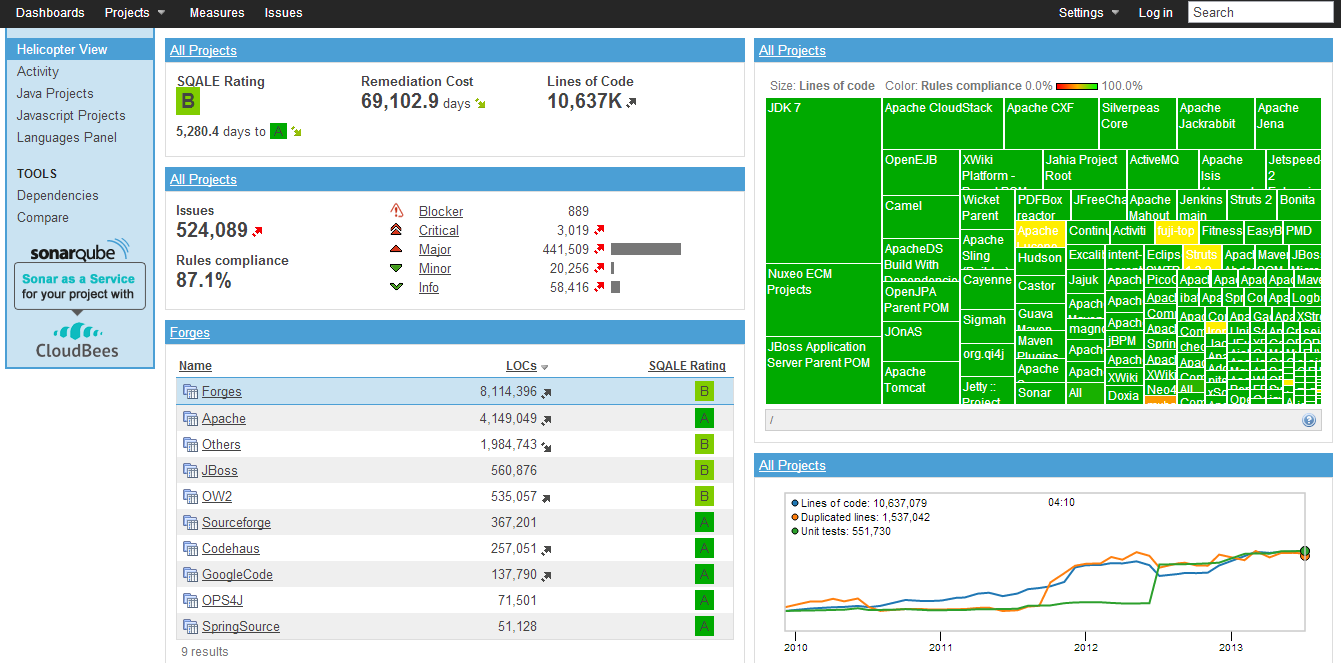
\includegraphics[scale=0.3]{images/SonarQube.png}
      \end{center}
      \caption{Exemple d'un rapport d'analyse statique de code fournit par SonarQube}
      \label{SonarQube}
    \end{figure}

    \subsection{Automatisation des tests et de la couverture de code}
    L'exécution des tests, par le biais de framework, est propres à chaque langage et à chaque équipe de travail. En javascript par exemple, les tests unitaires peuvent mise en place avec Moccha, Jasmine, Unitjs... Le serveur d'Intégration Continue ne fait qu'automatiser leur lancement à chaque commit du code source et disposer d'un affichage graphique des résultats via le plugin JUnit Plugin. Pour cela le framework de test doit fournir en sortie un rapport au format XML (Voir Figure \ref{ReportXML}) qui sera interprété par le plugin JUnit.

    \begin{figure}
      \begin{center}
        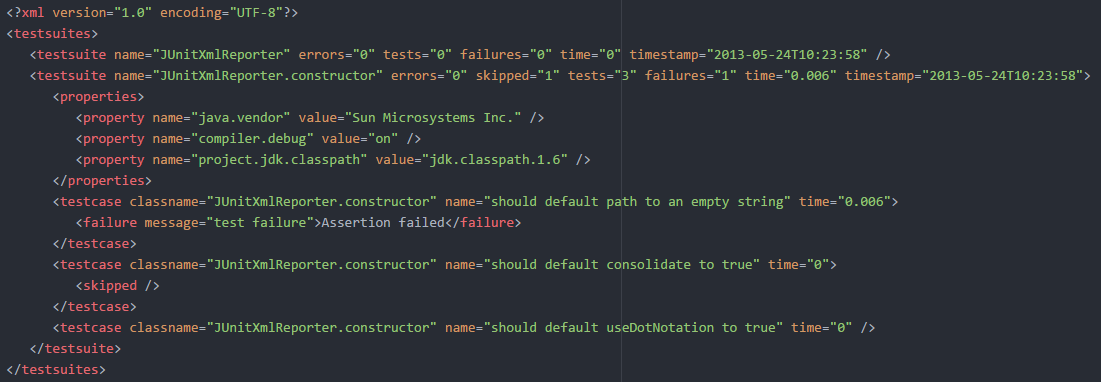
\includegraphics[scale=0.5]{images/ReportXML.png}
      \end{center}
      \caption{Exemple d'un rapport de test au format XML d'une application Java}
      \label{ReportXML}
    \end{figure}

    \subsection{Documentation Continue}
    Les équipes de développement d'AXA ne sont soumis à aucune politique de documentation du code source. Libre à chacun de documenter ou non son développement. De ce fait, la Documentation Continue ne fait pas partie des fonctionnalités de notre plate-forme d'Intégration Continue.

    \subsection{Déploiement Continu}
    Officiellement AXA possède quatre environnements dans le cycle de de développement d'une application; l'environnement de développement, l'environnement de recette (ou de qualification), l'environnement de pré-production et celui de production. De plus la DSI d'AXA France subit une profonde transformation digitale poussée par l'émergence du Cloud. Une forte volonté de migration des applications AXA dans le cloud est présente. Cependant la migration étant longue et encore en phase de test, peu d'applications sont hébergées dans le Cloud ce qui implique le maintient d'une infrastructure physique. Le Déploiement Continue au sein d'AXA doit donc prendre en compte 4 environnements ainsi que deux types d'architectures serveur.\\

    L'infrastructure serveur de la DSI d'AXA est gérée par un prestataire de service interne à AXA - AXA Tech. Les développeurs n'ont ainsi qu'une très faible marge d'action sur la gestion des divers environnements. Le Déploiement Continue est ainsi possible sur les trois premiers environnements (développement, recette, pré-production). Le déploiement sur les instances de production est fait manuellement lors de mises en production (MEP) éparses.\\

    L'utilisation de la technologie des conteneurs (Voir la section \ref{Containers}) n'est encore que trop peu développée au sein d'AXA faute de non compatibilité des serveurs.

      \subsubsection{La gestion des dépendances}\label{Nexus}
      Lors du développement d'une application de nombreuses dépendances sont utilisées. A AXA, la gestion de ces dernières est effectuée par le gestionnaire de dépendance (ou repository manager) Nexus, qui permet de répondre à deux problématiques; il agit comme un proxy entre AXA et les dépôts publics et permet d'organiser la localisation des déploiements des dépendances spécifiques à l'entreprise.\\

      Fournir un proxy (et en même temps un cache) aux dépôts publics distants permet d'accélerer le processus de build en évitant le téléchargement redondant des dépendances. Les dépendances ne seront téléchargées qu'une unique fois depuis internet et stockées au niveau du cache du repository manager. De plus il permet à l'organisation de contrôler les dépendances téléchargées ainsi que leur version, garantissant une uniformité des ces dernières.

      Le repository manager a aussi pour fonctionnalité de mettre à la disposition de l'entreprise un dépôt interne partagé où les binaires et autres artefacts générés peuvent être entreposés et versionnés.\\

    \subsection{Feedback Continue}
    Notre plate-forme d'Intégration Continue Jenkins utilise les emails comme chaine de rétroaction primaire. Les rapports par mail sont très faciles à mettre en place. Du côté de la configuration, Jenkins envoie des emails après chaque build échouée et en cas de changement d'état de construction. Nous avons également inclus l'identité du dernier développeur à avoir cassé ou réparé la build afin de favoriser la collaboration des divers acteurs. Les adresses mails des bénéficiaires sont prédéfinies et les équipes de travail sont déterminer afin de faciliter la gestion de la rétroaction par email.\\

    Nous utilisons l'interface web de Jenkins comme chaine de feedback secondaire. Hautement disponible, elle fournit l'intégralité des données nécéssaires à à la rétroaction et permet aux équipes d'avoir une vue générale de l'état des différentes builds de leurs applications.

  \section{Architecture}

    \subsection{Serveur d’Intégration Continue}

    \subsection{Logiciel de gestion de configuration}

    \subsection{Réseaux et déploiement}

  \section{Configuration}

    \subsection{« Build Jobs »}

      \subsubsection{Découpage des jobs}
      Plus l'exécution d'une build est longue, plus le temps de la rétroaction augmente. Or un des objectifs de l'Intégration Continue est de minimiser cette rétroaction. Cinq minutes, est le seuil maximal défini par AXA pour la réalisation d'un Job. Si un Job prend plus de temps, il est nécessaire de la découper en plusieurs étapes consécutives. Jenkins est designé pour permettre le déclenchement des Jobs les un après les autres. Il est donc facile de détailler une construction lourde en plusieurs petites étapes, favorisant la rétroaction après chaque étape sans avoir à attendre la fin de la construction. \\

      Nous ne pouvons pas définir de découpage générique à toutes les applications présentes dans la PIC AXA; trop de paramètres entrent en compte. En revanche nous pouvons décrire une séquence type, illustrative d'un worflow d'Intégration Continue. Les jobs s'exécutant séquentiellement si et seulement si le précédent est un succès. Le premier Job lancé est l'inspection statique du code source, suivi de la compilation, des tests, du packaging et du déploiement. Les tests, de part leur temps d'exécution, sont eux aussi découpés en plusieurs Jobs. Les tests unitaires, étant la première couche dans la hiérarchie des tests et la plus rapide à exécuter, ouvrent le bal.

      \subsubsection{Etablir des relations}
      Le déclenchement séquentiel des Jobs, les uns après les autres, peut également être utilisé pour gérer les dépendandes de construction. Si un module logiciel A dépend d'un module B et C, la construction de A peut être déclenchée si la build d'une des dépendances est exécutée. Jenkins met en place un mécanisme d'upstream (amont) et de downstream (aval) pour les relations de dépendance. Quelques fois les équipes de développement effectuent plusieurs commits sur un module logiciel unique dans un court laps de temps, afin de diviser l'intégration en petits lots commentés. En pratique tous ces commits peuvent être interprétés comme un seul. Pour éviter le déclenchement de builds upstream ou downstream Jenkins introduit une période de silence. Si une build est configurée pour avoir cinq minutes de période de silence, elle est mise en attente lorsqu'elle est déclenchée et ne s'exécute que si aucun autre commit à eu lieu sur le module pendant ce laps de temps. Sinon la période de silence est de nouveau repoussée à cinq minutes.\\

      Jenkins peut également être configuré pour éviter les déclenchements downstream (aval) des builds pendant l'exécution d'une build upsteam (amont).

    \subsection{Reporting}
    Pour chaque build nous générons automatiquement différents rapports à l'aide des fonctionnalités et plugins intégrés à Jenkins. Nous recueillons ainsi les résultats des tests et de la couverture de code (pour les tests unitaires). D'après les résultats, l'interface web de Jenkins génère des graphiques de tendance, qui visualise la quantité de tests passants et non-passants au fil du temps (Voir la Figure \ref{JenkinsTestReport}). Il est également possible de visualiser les résultats d'un test particulier. AXA configure ses builds pour conserver un historique sur trente exécutions.\\

    \begin{figure}
      \begin{center}
        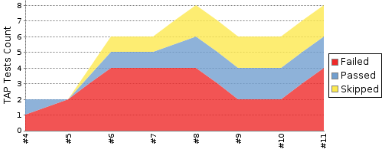
\includegraphics[scale=1]{images/JenkinsTestReport.png}
      \end{center}
      \caption{Exemple d'un graphique de tendance des tests unitaires dans Jenkins}
      \label{JenkinsTestReport}
    \end{figure}

    Les violations de conventions de codage sont également enregistrées. Avec le plugin adéquat, le rapport présenté dans Jenkins nous montre visuellement le nombre de violations ayant eu lieu ainsi que leur gravité (Voir la Figure \ref{JenkinsCodingReport}). Nous disposons même d'une vue de navigation où les lignes en violation sont surlignées dans le code source.\\

    \begin{figure}
      \begin{center}
        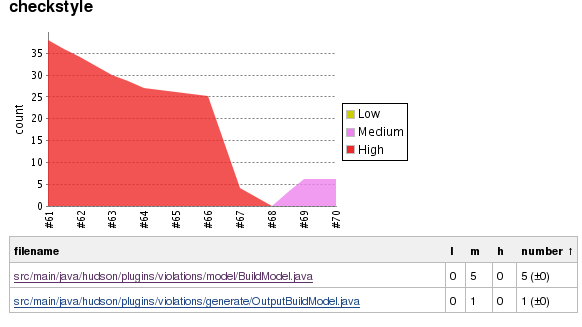
\includegraphics[scale=0.7]{images/JenkinsCodingReport.png}
      \end{center}
      \caption{Exemple d'un graphique de violation de convention de codage dans Jenkins}
      \label{JenkinsTestReport}
    \end{figure}

    La complexité du code source est également inclue dans les rapports de construction, permettant un refactoring rapide et garantissant une qualité de code.

  \section{Délivrables et artéfacts de build}
  Le type de délivrable attendu dépendra essentiellement du langage de l'application, de votre infrastructure et de la politique de déploiement de votre compagnie. A AXA, les applications Java sont packagées en war, les application .NET en msi et les applications Javascript en zip. Les containeurs ne sont pas encore utilisés au sein d'AXA, faute de non compatibilité de nos serveurs. L'intégralité de ces artefacts est archivé et versionné dans notre repository manager Nexus (dans le cadre de notre PIC Java/Javascript, pour la PIC .NET nous utilisons TFS).\\

  Ces délivrables sont nos principaux artéfacts de build, mais notre Intégration Continue produit également de la documentation, des changelogs et des rapports de build (vus dans la section précédente). En fonction de leur nature ils sont archivés et versionnés directement dans notre gestionnaire de code source ou dans Jenkins.\\

  \section{Observations et conclusion}
    \subsection{Point de départ}
    Avant la mise en place de l'Intégration Continue à AXA il n'y avait pas de processus abordant l'assurance de la qualité à tout niveau. La responsabilité de celle-ci était à la charge du développeur, dictée par son professionnalisme et sa motivation. Il était à la décision de chacun de tester son application avant qu'elle ne soit mise en production. Les étapes de compilation, de packaging et de déploiement étaient manuelles, ce qui demandait une charge de travail rébarbative et source d'erreur aux équipes de développement. Les déploiements étaient sporadiques et trop éloignés dans le temps conduisant à des mises en production douloureuses. Doublement éprouvant, que pour la mise en production, les équipes de travail d'AXA doivent passer par AXA Tech, le prestataire interne de notre infrastructure.\\

    \subsection{Les méthodes de travail}
    La majorité des développeurs présents à AXA ont eu une expérience de travail sans Intégration Continue. Le passage à l'Intégration Continue a changé leur façon de travailler et pour beaucoup d'entre eux avec un impact bénéfique. Même les développeurs qui n'étaient pas au courant de l'intégralité des règles de l'Intégration Continue vu dans la section \ref{Developers} ont pu facilement s'adapter à cette nouvelle méthodologie de travail; cela étant dû à leur bon sens.

      \subsubsection{Commiter les changements}
      Tous les développeurs passés à l'Intégration Continue synchronisent au moins quotidiennement leur changement avec le dépôt de code source. Leur fréquence depend de la tâche sur laquelle ils travaillent. S'ils développent une nouvelle fonctionnalité la fréquence d'intégration est plus faible que s'ils résoudent un bug ou effectuent une réfactorisation. Leur fréquence de commit correspond aux tâches agiles qu'ils effecuent - une tâche entraine irrémédiablement un commit.

      \subsubsection{Les tests locaux}
      L'une des étapes du cycle de travail de l'Intégration Continue est d'exécuter localement les tests avant d'intégrer leurs changements au dépôt partagé. Cependant nous constatons que certains développeurs n'exécutent les tests en local que lors de l'échec de leur build, mentionnant que puisque le serveur d'Intégration Continue les exécute eux ne le doivent pas. Dans d'autre cas, les développeurs ne sont pas en mesure d'effectuer les tests en local ne disposant pas de l'environnement nécessaire.

      \subsubsection{Usage des rapport et de la rétroaction}
      L'un des avantages de l'Intégration Continue est d'améliorer la visibilité des problèmes liée à la construction de artefacts de l'application (Voir la section \ref{Benefits}). Toutes les personnes que j'ai pu interroger ont indiqué qu'il était facile de trouver les informations liées à la santé d'une build. Les informations sont centralisées et standardisées au niveau du serveur d'Intégration Continue. Le point le plus intéressant de ces rapports et l'état général des constructions - échec ou succès. En cas d'échec le premier rapport est fourni par le message de sortie de la console du serveur.\\

      Les rapports de tests générés sont généralement peu utilisés car il nécessite une navigation au travers de plusieurs écrans tandis que la même information est présente dans le rapport précédent.\\

      Les rapports de code des analyseurs statiques sont très utiles aux développeurs. Ils standardisent les morceaux de code de chacun, renseignent sur les besoins de refactoring, et indiquent l'absence de documentation.\\

      Les retours par emails effectués par le serveur d'Intégration Continue sont généralement suivis même si quelques développeurs ont mentionné le fait que l'email n'était pour eux pas une bonne solution. Certains ont classé ces emails comme spams tandis que d'autres utilisent très peu leur boite de messagerie. Il a égalemment été évoqué que lorsqu'une build échoue à cause d'un problème autre qu'une erreur de programmation (problème d'installation par exemple) le rapport ne stipule pas clairement que le code poussé par le développeur est correct. Ce genre de problème et le manque de robustesse dans les builds réduisent un peu le profit de la rétroaction.\\

      En dépit des problèmes liés à la rétroaction, on constate que lorsqu'un problème a été identifié il est fixé le plus tôt possible.

      \subsubsection{Configuration des builds d'Intégration Continue}
      Les deux plate-formes d'Intégration Continue mise en place par AXA sont gérées exclusivement par une équipe dédiée. Ce qui pose problème à certaines équipes de développeurs qui souhaiteraient être maître de la configuration de leur build. De plus la demande de création et de configuration d'un pipeline de déploiement suit un processus lent et complexe composé d'une multitude d'intervenants ne favorisant pas l'agilité dans la création de projet. Ce qui induit que de nombreux projets ne bénéficie pas encore de l'infrastructure nécessaire à la pratique de l'Intégration Continue

    \subsection{Les bénéfices constatés}
    Le packaging automatique et le déploiement facile est la principale caractéristique de l'Intégration Continue. Réduire le workflow fastidieux du déploiement d'une application en une ligne de commande augmente considérablement le temps ainsi que l'humeur des développeurs. Outre les bénéfices pour le développeur l'automatisation améliore la qualité de l'intégration et de la livraisons en évitant toute erreur d'inattention et réduisant le temps de de déploiement.\\

    L'intégralité des développeurs ont mentionné que l'un des principaux avantages est l'automation des tests. Pour chaque changement apporté au code source la totalité des tests sont exécutés et si ne serait-ce qu'un test se révèle être défaillant aucune nouvaux packages est créé et le code poussé n'est pas incorporé au code source partagé. Les problèmes sont déclarés rapidemment et n'impactent qu'un seul développeur. Nous garantissons ainsi la propreté et la qualité du code source.\\

    Un autre bénéfice constaté est la gestion des builds de développement et de release. Le serveur d'Intégration Continue, aidé de ses plugins, marque les différents artefacts produit en fonction de leur version et de leur environnement. Cela permet de conserver un historique des builds et d'éviter l'installation de mauvais package.\\

    \subsection{Les axes d'amélioration}
    La PIC Jenkins, quoique remplissant parfaitement son rôle, n'est pas parfaite. Le premier axe à prendre en compte est son aspect centralisé. Les équipes de développement ont exclusivement les droits d'exécution et ne peuvent ainsi interagir dans la personnalisation de leurs pipelines de déploiement. Une équipe spécialisée est chargée de la configuration et de la gestion des Jobs pour l'ensemble de l'organisation. Victime de son succès l'Intégration Continue fait de plus en plus d'adepte au sein d'AXA ce qui accroisse la demande au niveau de la PIC. Les délais de disponibilité des nouveaux Jobs, parfois longs, continuent d'augmenter, ce qui nuit fondamentalement à la philosophie de l'Intégration Continue.\\

    Bien qu'étant une décision politique plus que technique, le maintient de deux plate-formes, pour un résultat similaire, peut-être considéré comme une perte de temps et d'argent. Il serait intéressant de fusionner les PIC Java/Javascript et .NET afin de ne disposer que d'un seul type d'infrastructure. \\

    Avec l'essor du Cloud, un autre axe d'amélioration serait de « cloudifier » nos plate-formes d'Intégration Continue afin de bénéficier du concept ATAWAD - « AnyTime, AnyWhere, AnyDevice » (tous le temps, depuis n'importe où, sur n'importe quel device) - et de réduire les coûts d'infrastructure.\\

    D'après les temoignages de développeurs travaillant en Intégration Continue sur les PIC AXA, la rétroaction des builds par email et par l'interface du serveur ne correspond pas à leurs attentes. La communication entre les collaborateurs et l'outil d'Intégration est un axe à améliorer.
